\documentclass[tikz]{standalone}
\input{common/tikzBase}
\usetikzlibrary{shapes.misc,arrows.meta,fit,decorations.pathreplacing,matrix,patterns}
\newcommand{\maincode}{
            pid = fork(); \\
            if (pid == 0) \{ \\
            \hspace{.5cm} open new files; \\
            \hspace{.5cm} exec\ldots(\ldots); \\
            \hspace{.5cm} \ldots \\
            \} else if (pid > 0) \{ \\
            \hspace{.5cm} waitpid(pid,\ldots); \\
            \hspace{.5cm} \ldots \\
            \} \\
            \ldots
        }
\newcommand{\maincodeWait}{
            pid = fork(); \\
            if (pid == 0) \{ \\
            \hspace{.5cm} open new files; \\
            \hspace{.5cm} exec\ldots(\ldots); \\
            \hspace{.5cm} \ldots \\
            \} else if (pid > 0) \{ \\
            \hspace{.5cm} \myemph{waitpid(pid,\ldots)}; \\
            \hspace{.5cm} \ldots \\
            \} \\
            \ldots
        }
\newcommand{\maincodeFork}{
            pid = \myemph{fork()}; \\
            if (pid == 0) \{ \\
            \hspace{.5cm} open new files; \\
            \hspace{.5cm} exec\ldots(\ldots); \\
            \hspace{.5cm} \ldots \\
            \} else if (pid > 0) \{ \\
            \hspace{.5cm} waitpid(pid,\ldots); \\
            \hspace{.5cm} \ldots \\
            \} \\
            \ldots
        }
\newcommand{\maincodeOpenNew}{
            pid = fork(); \\
            if (pid == 0) \{ \\
            \hspace{.5cm} \myemph{open new files}; \\
            \hspace{.5cm} exec\ldots(\ldots); \\
            \hspace{.5cm} \ldots \\
            \} else if (pid > 0) \{ \\
            \hspace{.5cm} waitpid(pid,\ldots); \\
            \hspace{.5cm} \ldots \\
            \} \\
            \ldots
}
\newcommand{\altcode}{
            main() \{ \\
            \hspace{.5cm} \ldots \\
            \}
}
\begin{document}

\setSlide{1}
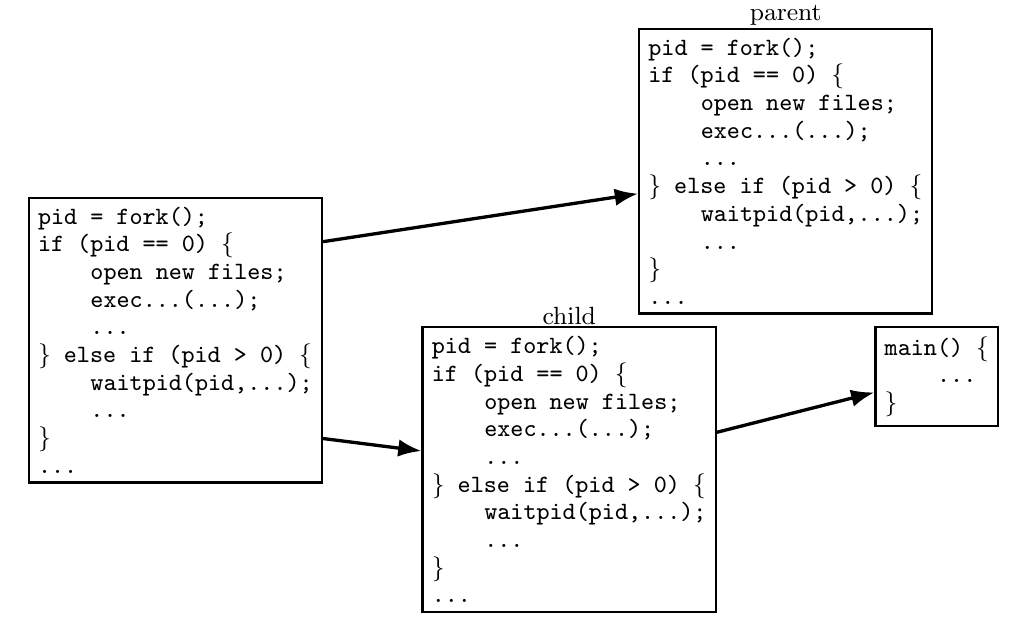
\begin{tikzpicture}
\tikzset{
    code box/.style={draw,thick,font=\tt\fontsize{9}{10}\selectfont,align=left},
    with the code/.style={
        code box,
    },
    with the other code/.style={
        code box,
    }
}
\node[with the code] (start) {\maincodeFork};
\node[with the code,anchor=south west,
      label={[font=\small,label distance=-1mm,overlay]north:parent}] (parent first) at ([xshift=4cm,yshift=-1.5cm]start.north east) {\maincodeWait};
\node[with the code,anchor=north west,
      label={[font=\small,label distance=-1mm]north:child}] (child first) at ([xshift=1.25cm,yshift=2cm]start.south east) {\maincodeOpenNew};
\node[with the other code,anchor=north west] (child second) at ([xshift=2cm]child first.north east) {\altcode};

\begin{scope}[very thick,>=Latex]
\draw[->] ([yshift=1.25cm]start.east) -- (parent first);
\draw[->] ([yshift=-1.25cm]start.east) -- (child first);
\draw[->] (child first) -- (child second);
\end{scope}
\end{tikzpicture}
\end{document}
